\renewcommand{\mydate}{2025年04月03号\ 第十二次课}

%\setcounter{framenumber}{30}
\makeatletter
\ifodd\value{page}
\else
\begin{frame}[plain]
\end{frame}
\fi
\makeatother

\section{线性空间}


\title{第六章 \quad 线性空间}
\author{}
\date{}

\frame{\titlepage}

\subsection{数组空间}





\subsubsection{$n$维数组空间}
\begin{frame}\frametitle{$n$维数组空间,线性相关性}
\begin{center}
空间 $\xrightarrow[1:1]{\text{坐标系}}$ $\bR^3$ $\xrightarrow{\text{推广}}$ $\bF^n=\bF\times \bF\times \cdots \times \bF$.
\end{center}
\pp
\begin{definition}
设$\bF$为数域. 带线性运算的$n$维数组向量全体
\[\{(a_1,a_2,\cdots,a_n)\mid a_i\in \bF\}\]
称为\blue{$n$维数组空间}.记为 $\bF^n$.
\end{definition}

\pp

\blue{线性组合(组合系数,线性表示)}

\pp

\begin{definition}[线性相关,线性无关]
一组向量 $\vec{a}_1$, $\vec{a}_2$, $\cdots$, $\vec{a}_m$ 称为\blue{线性相关}, 若存在一组不全为零的实数 $\lambda_1$, $\lambda_2$, $\cdots$, $\lambda_m$ 使得
\[\lambda_1\vec{a}_1 + \lambda_2\vec{a}_2 + \cdots + \lambda_m\vec{a}_m=0.\]
反之,	则称向量 $\vec{a}_1$, $\vec{a}_2$, $\cdots$, $\vec{a}_m$的\blue{线性无关}.
\end{definition}
\end{frame}



\subsubsection{子空间}
\begin{frame}\frametitle{子空间}
\pp
给定空间中的$m$个向量$\vec{a}_1,\vec{a}_2,\cdots,\vec{a}_m$.
\pp
考虑这$m$个向量的全体线性组合
\[V:=\langle\vec{a}_1,\vec{a}_2,\cdots,\vec{a}_m\rangle:=\{\lambda_1\vec{a}_1+\lambda_2\vec{a}_2+\cdots+\lambda_m\vec{a}_m\mid \lambda_1,\cdots,\lambda_m\in \bF\}\]
\pp
这是$\bF^n$的一个非空子集满足
\begin{enumerate}
\item 任取$\vec{b}_1$, $\vec{b}_2\in V$,都有$\vec{b}_1+\vec{b}_2\in V$;
\pp
\item 任取$\vec{b}\in V$以及$\lambda\in \bF$,都有$\lambda\vec{b}\in V$.
\end{enumerate}
\pp
上面两条也等价于
\begin{enumerate}\setcounter{enumi}{2}
\item 任取$\vec{b}_1$, $\cdots$, $\vec{b}_\ell\in V$以及$\mu_1,\cdots,\mu_\ell$,都有$\mu_1\vec{b}_1+\cdots+\mu_\ell\vec{b}_\ell\in V$.
\end{enumerate}
\pp
\begin{definition}
设$V$为$\bF^n$的一个非空子集.若$V$满足上述前两条或第三条,则称$V$为$\bF^n$的\blue{子空间}.
\end{definition}
\pp
子空间可看成是\blue{三维空间中过原点的线和平面在高维时的推广}.
\end{frame}




\renewcommand{\mydate}{2025年04月08号\ 第十三次课}


\subsubsection{子空间的例子}
\begin{frame}\frametitle{子空间的例子}

\begin{example}[平凡子空间]
$V=\{0\}$或$V=\bF^n$.
\end{example}
\pp
\begin{example}[生成子空间]
$\langle\vec{a}_1,\vec{a}_2,\cdots,\vec{a}_m\rangle$ 由$\vec{a}_1,\vec{a}_2,\cdots,\vec{a}_m$生成的子空间.
\end{example}

\pp

特别地，给定一个阶矩阵$A\in\bF^{m\times n}$,则其所有列向量可生成 $\bF^m$的一个子空间，其所有行向量可生成$\bF^n$的一个子空间。
\pp

\begin{example}[用子空间的观点来理解线性方程组]
设$A=(\vec{a}_1,\cdots,\vec{a}_m)$. 则 $Ax=\vec{b}$ 有解当且仅当 $\vec{b}\in \langle\vec{a}_1,\vec{a}_2,\cdots,\vec{a}_m\rangle$.
\end{example}
\pp

\begin{example}[齐次线性方程组的解空间]
$n$个变元的齐次线性方程组的解空间为$\bF^n$的一个子空间.
\end{example}
\end{frame}





\subsubsection{与线性映射相关的子空间}
\begin{frame}\frametitle{与线性映射相关的子空间}

\begin{example}[线性映射的像(image)]
设$\mA\colon \bF^n\rightarrow \bF^m$为一个线性映射.则
\[\mathrm{im}(\mA):=\{\mA(\vec{x}) \mid \vec{x}\in \bF^n\} \subseteq \bF^m\]
为$\bF^m$的一个子空间。称为线性映射$\mA$的\blue{像}.
\end{example}
\pp

\begin{example}[线性映射的核(kernel)]
设$\mA\colon \bF^n\rightarrow \bF^m$为一个线性映射.则
\[\ker(\mA):=\{\vec{x} \in \bF^n \mid \mA(\vec{x})=0\} \subseteq \bF^n\]
为$\bF^n$的一个子空间。称为线性映射$\mA$的\blue{核}.
\end{example}
\end{frame}





\subsection{线性相关性}

\subsubsection{线性相关等价刻画}
\begin{frame}\frametitle{线性相关等价刻画}
给定一组(列)向量 $\vec{a}_1$, $\vec{a}_2$, $\cdots$, $\vec{a}_m$. 则以下几条相互等价:
\begin{enumerate}
\item $\vec{a}_1$, $\vec{a}_2$, $\cdots$, $\vec{a}_m$ 线性相关;
\pp
\bigskip

\item 存在$i\in\{1,\cdots,m\}$以及$\lambda_1\cdots\lambda_{i-1},\lambda_{i+1},\cdots,\lambda_m\in \bF$ 使得
\[\vec{a}_i=\lambda_1\vec{a}_1 + \cdots+ \lambda_{i-1}\vec{a}_{i-1}  +\lambda_{i+1}\vec{a}_{i+1} + \cdots + \lambda_m\vec{a}_m;\]
\pp
\bigskip

\item 存在$i\in\{1,\cdots,m\}$ 使得
\[\vec{a}_i \in \langle \vec{a}_1,\cdots,\vec{a}_{i-1},\vec{a}_{i+1},\cdots,\vec{a}_m\rangle;\]
\pp
\bigskip

\item 存在$i\in\{1,\cdots,m\}$使得
\[\langle \vec{a}_1,\vec{a}_{2},\cdots,\vec{a}_m\rangle = \langle \vec{a}_1,\cdots,\vec{a}_{i-1},\vec{a}_{i+1},\cdots,\vec{a}_m\rangle;\]
\pp
\bigskip

\item 线性方程组 $AX=0$有非零解, 其中 $A=(\vec{a}_1,\vec{a}_{2},\cdots,\vec{a}_m)$;
\pp
\bigskip

\item $A$不是列满秩;
\pp
\bigskip

\item $\det(A)=0$ (当$m=n$时).
\end{enumerate}
\end{frame}






\subsubsection{线性无关等价刻画}
\begin{frame}\frametitle{线性无关等价刻画}
给定一组(列)向量 $\vec{a}_1$, $\vec{a}_2$, $\cdots$, $\vec{a}_m$. 则以下几条相互等价:
\begin{enumerate}
\item $\vec{a}_1$, $\vec{a}_2$, $\cdots$, $\vec{a}_m$ 线性无关;
\pp
\bigskip

\item 任取$i\in\{1,\cdots,m\}$以及$\lambda_1\cdots\lambda_{i-1},\lambda_{i+1},\cdots,\lambda_m\in \bF$,
\[\vec{a}_i\neq\lambda_1\vec{a}_1 + \cdots+ \lambda_{i-1}\vec{a}_{i-1}  +\lambda_{i+1}\vec{a}_{i+1} + \cdots + \lambda_m\vec{a}_m;\]
\pp
\bigskip

\item 任意$i\in\{1,\cdots,m\}$,
\[\vec{a}_i \notin \langle \vec{a}_1,\cdots,\vec{a}_{i-1},\vec{a}_{i+1},\cdots,\vec{a}_m\rangle;\]
\pp
\bigskip

\item 任意$i\in\{1,\cdots,m\}$,
\[\langle \vec{a}_1,\vec{a}_{2},\cdots,\vec{a}_m\rangle \neq \langle \vec{a}_1,\cdots,\vec{a}_{i-1},\vec{a}_{i+1},\cdots,\vec{a}_m\rangle;\]
\pp
\bigskip

\item 线性方程组 $AX=0$无非平凡解, 其中 $A=(\vec{a}_1,\vec{a}_{2},\cdots,\vec{a}_m)$;
\pp
\bigskip

\item $A$为列满秩;
\pp
\bigskip

\item  $\det(A)\neq 0$ (当$m=n$时).
\end{enumerate}
\end{frame}






\begin{frame}\frametitle{例子}

\begin{example}
包含零向量的任意向量组线性相关.
\end{example}
\pp

\begin{example}
设$S_1,S$为$\bF^n$的两个有限子集满足 $S_1\subseteq S$.
\pp
则
\begin{enumerate}
\item $S_1$线性相关 $\Rightarrow$ $S$线性相关;
\pp
\item $S$线性无关 $\Rightarrow$ $S_1$线性无关;
\end{enumerate}
\end{example}

\pp
\begin{example}[判定下列向量组的线性相关性]
\begin{enumerate}
\item $\vec{e}_1,\vec{e}_2,\cdots,\vec{e}_n$单位坐标向量.
\pp
\item $\vec{a}_1=(1,0,0,\cdots,0)^T$, $\vec{a}_2=(1,1,0,\cdots,0)^T$, $\cdots$, $\vec{a}_n=(1,1,1,\cdots,1)^T$.
\pp
\item $\vec{a}_1+\vec{a}_2$, $\vec{a}_2+\vec{a}_3$, $\vec{a}_3+\vec{a}_1$,其中 $\vec{a}_1,\vec{a}_2,\vec{a}_3$线性无关.
\pp
\item $\vec{a}_1=(3,4,-2,5)^T$, $\vec{a}_2=(2,-5,0,-3)^T$, $\vec{a}_3=(5,0,-1,2)^T$, $\vec{a}_4=(3,3,-3,5)^T$.
\end{enumerate}
\end{example}
\end{frame}





\subsubsection{线性映射与线性相关性}
\begin{frame}\frametitle{线性映射与线性相关性}

\begin{proposition}
任意给定一个线性映射$\mA\colon \bF^n \rightarrow \bF^m$. 对$\bF^n$中任意有限个向量 $\vec{a}_1, \vec{a}_2, \cdots, \vec{a}_m$, \pp 都有
\begin{enumerate}
\item $\vec{a}_1,\vec{a}_2,\cdots,\vec{a}_m$ 线性相关 $\Rightarrow$ $\mA(\vec{a}_1),\mA(\vec{a}_2),\cdots,\mA(\vec{a}_m)$ 线性相关;
\item $\mA(\vec{a}_1),\mA(\vec{a}_2),\cdots,\mA(\vec{a}_m)$ 线性无关 $\Rightarrow$  $\vec{a}_1,\vec{a}_2,\cdots,\vec{a}_m$线性无关;
\pp
\end{enumerate}


\end{proposition}
\pp
\begin{example}[投影]
给定$m$个$r$维数组向量 $\vec{a}_i=(a_{i1},\cdots,a_{ir})\in \bF^r$ ($i=1,\cdots,m$). 将每个向量都扩充为一个$n$维向量 $\vec{b}_i = (a_{i1},\cdots,a_{ir},a_{ir+1},\cdots,a_{in})\in \bF^n$. \pp 则
\begin{enumerate}
\item $\vec{a}_1,\vec{a}_2\cdots,\vec{a}_m$线性无关 $\Rightarrow$ $\vec{b}_1,\vec{b}_2\cdots,\vec{b}_m$线性无关;
\item $\vec{b}_1,\vec{b}_2\cdots,\vec{b}_m$线性相关 $\Rightarrow$ $\vec{a}_1,\vec{a}_2\cdots,\vec{a}_m$线性相关;
\end{enumerate}
\end{example}
\end{frame}








\subsection{极大无关组}





\subsubsection{极大无关组}
\begin{frame}\frametitle{极大无关组}
\begin{definition}[极大无关组]
设$\vec{a}_1$, $\vec{a}_2$, $\cdots$, $\vec{a}_m$为一组向量.若子向量组$\vec{a}_{i_1}$, $\vec{a}_{i_2}$, $\cdots$, $\vec{a}_{i_r}$线性无关,且任加另一个向量$\vec{a}_{i_{r+1}}$后,向量组$\vec{a}_{i_1}$, $\vec{a}_{i_2}$, $\cdots$, $\vec{a}_{i_{r+1}}$线性相关,则称$\vec{a}_{i_1}$, $\vec{a}_{i_2}$, $\cdots$, $\vec{a}_{i_r}$为$\vec{a}_1$, $\vec{a}_2$, $\cdots$, $\vec{a}_m$的\blue{极大无关组}.
\end{definition}
\pp
\begin{proposition}[通过生成子空间来判定极大无关组]
给定向量组$\vec{a}_1$, $\vec{a}_2$, $\cdots$, $\vec{a}_m$的一个子向量组$\vec{a}_{i_1}$, $\vec{a}_{i_2}$, $\cdots$, $\vec{a}_{i_r}$. 则$\vec{a}_{i_1}$, $\vec{a}_{i_2}$, $\cdots$, $\vec{a}_{i_r}$为$\vec{a}_1$, $\vec{a}_2$, $\cdots$, $\vec{a}_m$的极大无关组当且仅当
\begin{itemize}
\item $\vec{a}_{i_1}$, $\vec{a}_{i_2}$, $\cdots$, $\vec{a}_{i_r}$线性无关,且
\item $\langle \vec{a}_{i_1},\vec{a}_{i_2},\cdots,\vec{a}_{i_r}\rangle=\langle\vec{a}_1,\vec{a}_2,\cdots,\vec{a}_m\rangle$.
\end{itemize}
\end{proposition}
\end{frame}



\renewcommand{\mydate}{2025年04月10号\ 第十四次课}




\begin{frame}\frametitle{课本部分习题}
\begin{itemize}
\item[13.] 若向量组 $\boldsymbol{a}_1,\boldsymbol{a}_2,\cdots,\boldsymbol{a}_n\in F^n$ 线性无关，而 $\boldsymbol{a}_1,\boldsymbol{a}_2,\cdots,\boldsymbol{a}_n,\boldsymbol{b}$ 线性相关，则 $\boldsymbol{b}$ 可以表示成 $\boldsymbol{a}_1,\boldsymbol{a}_2,\cdots,\boldsymbol{a}_n$ 的线性组合，且表示唯一。
\pp
\bigskip

\item[14.] 证明向量表示基本定理：设 $\boldsymbol{a}_1,\boldsymbol{a}_2,\cdots,\boldsymbol{a}_n\in F^n$ 线性无关，则任意向量 $\boldsymbol{b}\in F^n$ 可以表示为 $\boldsymbol{a}_1,\boldsymbol{a}_2,\cdots,\boldsymbol{a}_n$ 的线性组合，且表示唯一。
\pp
\bigskip

\item[15.] 证明：非零向量组 $\boldsymbol{a}_1,\boldsymbol{a}_2,\cdots,\boldsymbol{a}_s$ 线性无关的充要条件是，每个 $\boldsymbol{a}_i(1 < i\leq s)$ 都不能用它前面的向量线性表示。
\pp
\bigskip

\item[16.] 设向量组 $\boldsymbol{a}_1,\boldsymbol{a}_2,\cdots,\boldsymbol{a}_s$ 线性无关， $\boldsymbol{b}=\lambda_1\boldsymbol{a}_1+\cdots+\lambda_s\boldsymbol{a}_s$ 。如 $\lambda_i\neq0$ ，则用 $\boldsymbol{b}$ 代替 $\boldsymbol{a}_i$ 后，向量组 $\boldsymbol{a}_1,\cdots,\boldsymbol{a}_{i - 1},\boldsymbol{b},\boldsymbol{a}_{i + 1},\cdots,\boldsymbol{a}_s$ 线性无关。
\pp
\bigskip

\item[17.] 设向量组 $\boldsymbol{a}_1,\boldsymbol{a}_2,\cdots,\boldsymbol{a}_r$ 线性无关，且 $\boldsymbol{a}_1,\boldsymbol{a}_2,\cdots,\boldsymbol{a}_r$ 可以由向量组 $\boldsymbol{b}_1,\boldsymbol{b}_2,\cdots,\boldsymbol{b}_r$ 线性表示，则 $\boldsymbol{b}_1,\boldsymbol{b}_2,\cdots,\boldsymbol{b}_r$ 也线性无关。
\end{itemize}
\end{frame}



% ========== 2023年04月18号 第13次课 极大无关组与秩 ==========
%\frame{\titlepage}





\subsubsection{极大无关组例子}
\begin{frame}\frametitle{极大无关组例子}
\begin{example}
证明$\vec{a}_1=(2,-1,3,1)$, $\vec{a}_2=(4,-2,5,4)$, $\vec{a}_3=(2,-1,4,-1)$中的任两个向量组成极大无关组.
\end{example}
\pp
\yang{$3\vec{a}_1=\vec{a}_2+\vec{a}_3$.}

\pp
注: 不唯一! 如何寻找极大无关组?一个一个去掉? \pp 比较麻烦! \pp 下面介绍简单方法.
\end{frame}





\subsubsection{寻找极大无关组的理论工具}
\begin{frame}\frametitle{寻找极大无关组的理论工具}
\pp
原理:初等行变换不改变列向量的线性相关性.
\pp
\begin{theorem}
设$\vec{a}_1$, $\vec{a}_2$, $\cdots$, $\vec{a}_m$为一组\blue{列}向量. \pp 对矩阵
\[A=(\vec{a}_1,\vec{a}_2,\cdots,\vec{a}_m)\in \bF^{n\times m}\]
做一系列\blue{行}初等变换得到
\[B=(\vec{b}_1,\vec{b}_2,\cdots,\vec{b}_m)\in \bF^{n\times m}.\]
\pp
则对于任意 $i_1,i_2,\cdots,i_r\in \{1,2,\cdots,m\}$,\pp
\begin{enumerate}
\item $\vec{a}_{i_1}$, $\vec{a}_{i_2}$, $\cdots$, $\vec{a}_{i_r}$线性相关(无关) $\Leftrightarrow$ $\vec{b}_{i_1}$, $\vec{b}_{i_2}$, $\cdots$, $\vec{b}_{i_r}$线性相关(无关); \pp
\item $\vec{a}_{i_1}$, $\vec{a}_{i_2}$, $\cdots$, $\vec{a}_{i_r}$极大无关 $\Leftrightarrow$ $\vec{b}_{i_1}$, $\vec{b}_{i_2}$, $\cdots$, $\vec{b}_{i_r}$极大无关;
\end{enumerate}
\end{theorem}

\yang{注：这个定理保证了行变换不改变列秩!}

\end{frame}






\begin{frame}\frametitle{证明}
\pp
\begin{equation*}
\begin{split}
(1) \qquad LHS \qquad \Leftrightarrow & AX=0 \text{ 有非零解} \\ \pp
\xLeftrightarrow[P\text{可逆}]{B=PA} & BX=0 \text{ 有非零解} \\ \pp
\Leftrightarrow & RHS.\\
\end{split}
\end{equation*}
\pp

\begin{equation*}
\begin{split}
(2) \qquad LHS \qquad \Leftrightarrow
& \left\{ { a_{i_1},\cdots, a_{i_r} \text{ 线性无关} \atop a_{i_1},\cdots, a_{i_r}, a_j\text{线性相关 $\forall$ $j$}}\right.\\ \pp
\xLeftrightarrow{(1)} & \left\{ { b_{i_1},\cdots, b_{i_r} \text{ 线性无关} \atop b_{i_1},\cdots, b_{i_r}, b_j\text{线性相关 $\forall$ $j$}}\right.\\ \pp
\Leftrightarrow & RHS.
\end{split}
\end{equation*}

\end{frame}






\begin{frame}\frametitle{寻找极大无关组例子}
\begin{example}
求向量组$\vec{a}_1=(-1,5,3,-2)$, $\vec{a}_2=(4,1,-2,9)$, $\vec{a}_3=(2,0,-1,4)$, $\vec{a}_4=(0,3,4,-5)$
\end{example}
\pp
\[
\begin{pmatrix}
-1& 4& 2& 0\\
5& 1& 0& 3\\
3& -2& -1& 4\\
-2& 9& 4& -5\\
\end{pmatrix}
\pp
\longrightarrow
\begin{pmatrix}
-1& 4& 2& 0\\
0& 1& 0& -5\\
0& 0& 5& 24\\
0& 0& 0& 0\\
\end{pmatrix}
\]
\pp
$\xRightarrow{\text{行变换}}$ $\{\vec{b}_1,\vec{b}_2,\vec{b}_3\}$,$\{\vec{b}_1,\vec{b}_2,\vec{b}_4\}$极大无关.\\
\pp
$\Rightarrow$ $\{\vec{a}_1,\vec{a}_2,\vec{a}_3\}$,$\{\vec{a}_1,\vec{a}_2,\vec{a}_4\}$极大无关.

\pp
\blue{问题:} 两个极大无关组的个数是否相等?
\begin{equation*}
\xymatrix{
& \vec{a}_{1},\vec{a}_{2}, \cdots, \vec{a}_{m} \ar[dr]\ar[dl] &\\
\{\vec{a}_{i_1}, \vec{a}_{i_2}, \cdots,\vec{a}_{i_r}\} && \vec{a}_{j_1}, \vec{a}_{j_2}, \cdots, \vec{a}_{j_s} \\
}
\end{equation*}
\end{frame}






\subsection{秩}


\subsubsection{等价向量组}
\begin{frame}\frametitle{等价向量组}
\pp
\begin{definition}[等价]
称两向量组$\vec{a}_1,\vec{a}_2,\cdots,\vec{a}_m$和$\vec{b}_1,\vec{b}_2,\cdots,\vec{b}_\ell$ \blue{等价},\pp 若
\begin{enumerate}
\item 任意$i\in\{1,\cdots,m\}$, $\vec{a}_i$可由$\vec{b}_1,\vec{b}_2,\cdots,\vec{b}_\ell$线性表示;\pp
\item 任意$i\in\{1,\cdots,\ell\}$, $\vec{b}_i$可由$\vec{a}_1,\vec{a}_2,\cdots,\vec{a}_m$线性表示;
\end{enumerate}
\pp
此时记为 \blue{$\{\vec{a}_1,\vec{a}_2,\cdots,\vec{a}_m\}\sim\{\vec{b}_1,\vec{b}_2,\cdots,\vec{b}_\ell\}$}.
\end{definition}
\pp
\begin{theorem}[通过生成子空间来判定是否等价]
\[\small \{\vec{a}_1,\cdots,\vec{a}_m\} \sim \{\vec{b}_1,\cdots,\vec{b}_\ell\} \quad \Leftrightarrow \quad \langle \vec{a}_1,\cdots,\vec{a}_m \rangle = \langle \vec{b}_1,\cdots,\vec{b}_\ell \rangle.\]
\end{theorem}
\pp
注: $\sim$为等价关系.
\pp
\begin{corollary}
\begin{enumerate}
\item 一个向量组与它的任一极大无关组等价; \pp
\item 任两极大无关组等价.
\end{enumerate}
\end{corollary}
\end{frame}





\subsubsection{极大无关组的基本性质与秩的定义}
\begin{frame}\frametitle{极大无关组的基本性质与秩的定义}

\begin{theorem}
设$\vec{a}_1,\vec{a}_2,\cdots,\vec{a}_r$和$\vec{b}_1,\vec{b}_2,\cdots,\vec{b}_s$为两线性无关的向量组. 若它们相互等价,则$r=s$.
\end{theorem}
\pp
\yang{证明思路: $\left\{{
(\vec{a}_1,\vec{a}_2,\cdots,\vec{a}_r) = (\vec{b}_1,\vec{b}_2,\cdots,\vec{b}_s)A_{s\times r}
\atop
(\vec{b}_1,\vec{b}_2,\cdots,\vec{b}_s)= (\vec{a}_1,\vec{a}_2,\cdots,\vec{a}_r)B_{r\times s}
}\right. \Rightarrow \left\{{
AB = I_s \atop BA = I_r
}\right. \Rightarrow r=s.$}
\pp
\begin{corollary}
向量组$\vec{a}_1,\vec{a}_2,\cdots,\vec{a}_m$的任两个极大无关组中的向量个数相同.这个数称为\blue{向量组的秩}.
记为\blue{$\rank(\vec{a}_1,\vec{a}_2,\cdots,\vec{a}_m)$}
或者\blue{$r(\vec{a}_1,\vec{a}_2,\cdots,\vec{a}_m)$}.
\end{corollary}
\pp
\begin{proposition}[用秩判定相关性]
\begin{enumerate}
\item $\vec{a}_1,\vec{a}_2,\cdots,\vec{a}_m$线性无关 $\Leftrightarrow$ $\rank(\vec{a}_1,\vec{a}_2,\cdots,\vec{a}_m)=m$;
\pp
\item $\vec{a}_1,\vec{a}_2,\cdots,\vec{a}_m$线性相关 $\Leftrightarrow$ $\rank(\vec{a}_1,\vec{a}_2,\cdots,\vec{a}_m)<m$;
\end{enumerate}
\end{proposition}
\end{frame}





\subsubsection{秩与线性相关性}
\begin{frame}\frametitle{秩与线性相关性}

\pp
\begin{theorem} 若$\vec{b}_1,\vec{b}_2,\cdots,\vec{b}_s$可由$\vec{a}_1,\vec{a}_2,\cdots,\vec{a}_r$线性表示,则
\[\rank(\vec{b}_1,\vec{b}_2,\cdots,\vec{b}_s)\leq
\rank(\vec{a}_1,\vec{a}_2,\cdots,\vec{a}_r).\]
\end{theorem}
\pp
\yang{证明思路:不妨设$\vec{a}_1,\vec{a}_2,\cdots,\vec{a}_\ell$ 和$\vec{b}_1,\vec{b}_2,\cdots,\vec{b}_k$为极大无关组.则
$(\vec{b}_1,\cdots,\vec{b}_k) = (\vec{a}_1,\cdots,\vec{a}_\ell) A$, 其中$A\in\bF^{\ell\times k}$列满秩.因此 $k\leq\ell$.}
\pp
\begin{corollary}
\begin{enumerate}
\item $\bF^n$ 中任意$n+1$个向量一定线性相关.
\pp
\item 若$\vec{b}_1,\vec{b}_2,\cdots,\vec{b}_s$可由$\vec{a}_1,\vec{a}_2,\cdots,\vec{a}_r$线性表示,则 $\{\vec{a}_1,\vec{a}_2,\cdots,\vec{a}_r\}\sim\{\vec{b}_1,\vec{b}_2,\cdots,\vec{b}_s\}$ $\Leftrightarrow$ $\rank(\vec{b}_1,\vec{b}_2,\cdots,\vec{b}_s) = \rank(\vec{a}_1,\vec{a}_2,\cdots,\vec{a}_r)$;
\end{enumerate}
\end{corollary}
\pp
\begin{corollary}[用秩来判定线性方程组是否有解]
$\vec{b}$为$\vec{a}_1,\vec{a}_2,\cdots,\vec{a}_r$的线性组合 $\Leftrightarrow$ $\rank(\vec{a}_1,\vec{a}_2,\cdots,\vec{a}_r)=\rank(\vec{a}_1,\vec{a}_2,\cdots,\vec{a}_r,\vec{b})$.
\end{corollary}
\end{frame}





\subsubsection{向量组的秩与矩阵的秩}
\begin{frame}\frametitle{向量组的秩与矩阵的秩}
\[A=(a_{ij})_{m\times n} = \begin{pmatrix}\vec{a}_1\\\vdots\\\vec{a}_m\\\end{pmatrix} = \begin{pmatrix}\vec{b}_1&\cdots&\vec{b}_n\\\end{pmatrix}\]
\pp
我们有如下三种秩:
\begin{enumerate}
\item $\rank(A)$ \qquad\qquad\qquad 矩阵$A$的秩;
\item $\rank(\vec{a}_1,\cdots,\vec{a}_m)$ \qquad 矩阵$A$的行秩;
\item $\rank(\vec{b}_1,\cdots,\vec{b}_n)$ \qquad 矩阵$A$的列秩;
\end{enumerate}
\pp
\begin{theorem}
\begin{center}
秩 = 行秩 = 列秩.
\end{center}
\end{theorem}

\pp

\yang{证明思路:初等变换不改变三者且对于标准形矩阵三者一致.}
\end{frame}






\renewcommand{\mydate}{2025年04月15号\ 第十五次课}





\subsubsection{矩阵秩的一些性质}
\begin{frame}\frametitle{矩阵秩的一些性质}
\begin{corollary}
设$A$为$n$阶方阵.
\pp
则
\begin{enumerate}
\item $A$可逆 $\Leftrightarrow$ $\rank(A)=n$ $\Leftrightarrow$ 行向量线性无关 $\Leftrightarrow$ 列向量线性无关.
\pp
\item $\rank(A)=r$ $\Rightarrow$ 不为零的$r$阶子式所在的行(列)构成的A的行(列)向量的极大无关组.
\end{enumerate}
\end{corollary}
\pp
\begin{example}
\[rank(AB)\leq \min\big(\rank(A),\rank(B)\big).\]
\end{example}
\end{frame}









% ========== 2023年04月20号 第14次课 基与维数 ==========
%\frame{\titlepage}





%











\subsection{基与维数}


\subsubsection{子空间的基与维数}
\begin{frame}\frametitle{子空间的基与维数}
\pp
\begin{theorem}
向量空间$\bF^n$的任意子空间都可以由有限个向量生成.
\end{theorem}
\pp
\yang{
证明思路: 反证.\pp 假若子空间$V$不能由有限个向量生成.\pp 则存在一列向量
\[a_1,a_2,a_3,\cdots\]
使得 $a_i \in V \setminus \langle a_1,\cdots,a_{i-1}\rangle$.\pp 特别地, (由习题15知)
\[a_1,\cdots,a_{n+1}\]
线性无关.\pp 矛盾!
}
\pp
\begin{corollary}
对于任意$\bF^n$的子空间$V$,存在一组线性无关的向量$\vec{a}_1,\cdots,\vec{a}_r$使得
\[V= \langle\vec{a}_1,\cdots,\vec{a}_r\rangle.\]
\end{corollary}
\end{frame}




\begin{frame}\frametitle{子空间的基与维数}
\pp
\begin{definition}[基]
设$V$为$\bF^n$的子空间.\pp 若向量组$\vec{a}_1,\cdots,\vec{a}_r$ \pp
\begin{itemize}
\item 线性无关,\pp 且
\item 生成子空间$V$,
\end{itemize}
\pp
则称$\vec{a}_1,\cdots,\vec{a}_r$为$V$的\blue{一组基}.\pp 称基中向量的个数$r$为子空间$V$的\blue{维数}.
\end{definition}

\begin{proposition}[坐标]
设向量组$\vec{a}_1,\cdots,\vec{a}_r$为$V$的一组基.\pp  则任意$\vec{a}\in V$可\blue{唯一}地表示为$\vec{a}_1,\cdots,\vec{a}_r$的线性组合.\pp 即,存在\blue{唯一}的一组数$\lambda_1,\cdots,\lambda_r\in \bF$使得 \[\tiny \vec{a}=\sum_{i=1}^r\lambda_i\vec{a}_i=:(\vec{a}_1,\cdots,\vec{a}_r)\begin{pmatrix}\lambda_1\\\vdots\\\lambda_r\end{pmatrix}.\]
\pp
称$(\lambda_1,\cdots,\lambda_r)$为$\vec{a}$在基$\{\vec{a}_1,\cdots,\vec{a}_r\}$下的\blue{坐标}.
\end{proposition}
\end{frame}



\subsubsection{扩充基}
\begin{frame}\frametitle{扩充基}

\begin{theorem}[扩充基]
设$V$为$\bF^n$的$r$维子空间.\pp 设$\vec{a}_1,\cdots,\vec{a}_s$为$V$中一组线性无关向量.\pp 则
$s\leq r$且存在$\vec{a}_{s+1},\cdots,\vec{a}_r\in V$ 使得$\vec{a}_1,\cdots,\vec{a}_r$构成$V$的一组基.\pp 称$\vec{a}_1,\cdots,\vec{a}_r$为$\vec{a}_1,\cdots,\vec{a}_s$的一组\blue{扩充基}.
\end{theorem}
\pp
\begin{proposition}
设$U$和$V$为$\bF^n$的两个子空间.\pp
\begin{enumerate}
\item 若$\dim(V)=r$,则$V$中的任意$r+1$个向量线性相关;\pp
\item 若$\dim(V)=r$且$\vec{a}_1,\cdots,\vec{a}_r\in V$线性无关,则$\{\vec{a}_1,\cdots,\vec{a}_r\}$为$V$的一组基.\pp
\item 若$U\subseteq V$,则$\dim U\leq \dim V$.\pp
\item 若$U\subseteq V$且$\dim U=\dim V$,则$U=V$.
\end{enumerate}
\end{proposition}
\end{frame}


\subsection{坐标与坐标变换}

\subsubsection{基与坐标}
\begin{frame}\frametitle{基与坐标}
\begin{example}[自然基] 称$\vec{e}_1,\cdots,\vec{e}_n$为$\bF^n$的自然基. 任意向量在自然基下的向量为自身,即
\[
\begin{pmatrix}b_1\\\vdots\\b_n\end{pmatrix}=(\vec{e}_1,\cdots,\vec{e}_n)\begin{pmatrix}b_1\\\vdots\\b_n\end{pmatrix}.
\]
\end{example}
\pp
\begin{equation*}
\boxed{\xymatrix@R=2mm{
\text{空间} \ar@{->}[r]^-{\text{坐标系}}_-{1:1} & \bR^3\\
\text{点} \ar@{|->}[r] & \text{点在坐标系下的坐标}\\
}}
\end{equation*}
\pp 推广
\begin{equation*}
\boxed{\xymatrix@R=2mm{
\text{$\bF^n$的$r$维子空间} \ar@{->}[r]^-{\text{\quad 基 \quad}}_-{1:1} & \bF^r\\
\text{向量} \ar@{|->}[r] & \text{向量在基下的坐标}\\
}}
\end{equation*}
\end{frame}





\subsubsection{坐标变换}
\begin{frame}\frametitle{坐标变换}
设$\vec{a}_1,\cdots,\vec{a}_r$和$\vec{b}_1,\cdots,\vec{b}_r$为$V$的两组基.\pp 设向量$v\in V$在两组基下的坐标分别为 $X=\begin{pmatrix}x_1\\\vdots\\x_r\end{pmatrix}$ 和$Y= \begin{pmatrix}y_1\\\vdots\\y_r\end{pmatrix}$.\pp 即,
\[v=(\vec{a}_1,\cdots,\vec{a}_r)X
=(\vec{b}_1,\cdots,\vec{b}_r)Y.\]
\pp
\blue{问题:} 如何确定$X$和$Y$之间的关系?
\end{frame}






\begin{frame}\frametitle{坐标变换}
\begin{proposition}
设$\vec{a}_1,\cdots,\vec{a}_r$和$\vec{b}_1,\cdots,\vec{b}_r$为$V$的两组基.\pp 则
\begin{enumerate}
\item 存在唯一$r$阶方阵$T$使得
\[(\vec{b}_1,\cdots,\vec{b}_r) = (\vec{a}_1,\cdots,\vec{a}_r)T.\]
\pp
矩阵$T$称为从基$\vec{a}_1,\cdots,\vec{a}_r$到基$\vec{b}_1,\cdots,\vec{b}_r$的\blue{过渡矩阵}.
\pp
\item 设向量$v\in V$在两组基下的坐标分别为 $X=\begin{pmatrix}x_1,&\cdots,&x_r\end{pmatrix}^T$ 和$Y= \begin{pmatrix}y_1,&\cdots,&y_r\end{pmatrix}^T$.\pp 则
\[X=TY.\qquad\text{\blue{(坐标变换公式)}}\]
\end{enumerate}
\end{proposition}
\pp
\blue{注:} 过渡矩阵$T$总是可逆的.
\end{frame}






\begin{frame}\frametitle{坐标变换例子}

\begin{example}
逆时针旋转平面直角坐标系$\theta$角.
\end{example}
\pp
\begin{equation*}
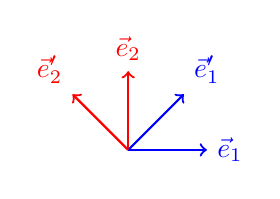
\begin{tikzpicture}[scale=0.5]
\coordinate (O) at (0,0);
\coordinate (X) at (2,0);
\coordinate (Y) at (0,2);
\coordinate (a) at (1.414,1.414);
\coordinate (b) at (-1.414,1.414);
\draw[->,thick,blue](O)--(X) node[pos=1,right] {$\vec{e}_1$};
\draw[->,thick,red](O)--(Y) node[pos=1,above] {$\vec{e}_2$};
\draw[->,thick,blue](O)--(a) node[pos=1,above right] {$\vec{e}'_1$};
\draw[->,thick,red](O)--(b) node[pos=1,above left] {$\vec{e}'_2$};
\end{tikzpicture}
\end{equation*}
\pp
$\Rightarrow (e_1',e_2') = (e_1,e_2)\begin{pmatrix}
\cos\theta&-\sin\theta\\\sin\theta&\cos\theta\\
\end{pmatrix}$
\pp
$\Rightarrow \begin{pmatrix} x\\y\\\end{pmatrix}= \begin{pmatrix}
\cos\theta&-\sin\theta\\\sin\theta&\cos\theta\\
\end{pmatrix}\begin{pmatrix} x'\\y'\\\end{pmatrix}.$
\pp
$\Rightarrow
\begin{pmatrix} x'\\y'\\\end{pmatrix}
= \begin{pmatrix}
\cos\theta&-\sin\theta\\\sin\theta&\cos\theta\\
\end{pmatrix}^{-1} \begin{pmatrix} x\\y\\\end{pmatrix}= \begin{pmatrix}
\cos\theta&\sin\theta\\-\sin\theta&\cos\theta\\
\end{pmatrix} \begin{pmatrix} x\\y\\\end{pmatrix}.$
\end{frame}








\subsection{线性方程组解集的结构}

\subsubsection{解空间}
\begin{frame}\frametitle{解空间}
\begin{example}
证明$V=\{(x_1,x_2,x_3)\in\bR^3\mid x_1+x_2+x_3=0\}$为$\bR^3$的子空间.求$V$的维数并找出其一组基.
\end{example}
\pp
\yang{通解: $X = t_1\begin{pmatrix} 1\\-1\\0\end{pmatrix} + t_2\begin{pmatrix} 1\\0\\-1\end{pmatrix}$.}
\pp
\begin{example}
证明 $W=\{(x_1,x_2,x_3)\in\bR^3\mid x_1+x_2+x_3=0,2x_1-x_2+x_3=3\}$不是$\bR^3$的子空间.
\end{example}
\pp
设$A\in \bF^{m\times n}$, $b\in \bF^m$为非零向量.\pp 则 \begin{enumerate}
\item $V:=\{X\in \bF^n\mid AX=0\}$为子空间;
\item $W:=\{X\in \bF^n\mid AX=b\}$不是子空间.
\end{enumerate}
接下来学习$V$和$W$更进一步地性质.
\end{frame}

%







\subsubsection{有(唯一)解的判定}
\begin{frame}\frametitle{有(唯一)解的判定}
\begin{theorem}
设$A\in \bF^{m\times n}$, $b\in \bF^m$.\pp 则
\begin{enumerate}
\item $AX=b$有解 $\Leftrightarrow$ $\rank(A)=\rank(A,b)$.\pp
\item $AX=b$有唯一解 $\Leftrightarrow$ $\rank(A)=\rank(A,b)=n$.
\end{enumerate}
\end{theorem}
\pp
\begin{example}
设$A\in \bF^{m\times n}$.\pp 则
\begin{enumerate}
\item $AX=0$一定有解;\pp
\item $AX=0$有非零解 $\Leftrightarrow$ $\rank(A)<n$ $\xLeftrightarrow{\text{若$A$为方阵}}$ $\det(A)=0$.
\end{enumerate}
\end{example}

\end{frame}





\subsubsection{齐次线性方程组的解空间}
\begin{frame}\frametitle{齐次线性方程组的解空间}
\pp
\begin{definition}[基础解系]
设$A\in \bF^{m\times n}$.\pp 称解空间\footnote{$V$也称为矩阵$A$的\blue{零空间}，记为\blue{$N(A)$}.}
\[V=\{X\in \bF^n\mid AX=0\}\]
的一组基为齐次线性方程组$AX=0$的一个\blue{基础解系}.
\end{definition}
\pp
\begin{theorem}[解空间大小]
\[\dim(V) = n-\rank(A).\]
\end{theorem}

\end{frame}









% ========== 2023年04月23号 第15次课 习题课 ==========


% ========== 2023年04月25号 第16次课 一般线性空间 ==========
%\frame{\titlepage}



\renewcommand{\mydate}{2025年04月17号\ 第十六次课}


\subsubsection{齐次线性方程组的解空间与线性映射的核*}
\begin{frame}\frametitle{齐次线性方程组的解空间与线性映射的核*}
\pp
给定矩阵$A\in\bF^{m\times n}$.\pp 通过$\mA(\vec{x}):=A\vec{x}$,我们可定义一个线性映射
\[\mA\colon \bF^n \rightarrow \bF^m.\]
\pp
\begin{proposition}
线性映射$\mA$的核正好为齐次线性方程组$AX=0$的解空间.\pp 即
\[\ker\mA = \{X\in \bF^n \mid AX=0\}.\]
\end{proposition}
\pp
此外,我们还有
\begin{proposition}
\begin{itemize}
\item 线性映射$\mA$的像由$A$的全体列向量生成;
\footnote{称$A$的列向量生成的子空间为$A$的\blue{列空间}.
类似地, 称$A$的行向量生成的子空间为$A$的\blue{行空间}.}
\pp
\item $\dim(\ker\mA) + \dim(\mathrm{im}\mA) = n$.
\end{itemize}
\end{proposition}
\end{frame}





\subsubsection{非齐次线性方程组的解空间}
\begin{frame}\frametitle{非齐次线性方程组的解空间}
如何描述非齐次线性方程组的解空间?
\pp
\[W:=\{X\in \bF^n\mid AX=b\}\]
$W$和$V$有什么联系?
\pp
基本事实:
\begin{itemize}
\item $\forall \alpha,\beta \in W$ $\Rightarrow$ $\alpha-\beta\in V$.\pp
\item $\forall \alpha\in W,\gamma\in V$ $\Rightarrow$ $\alpha+\gamma\in W$.
\end{itemize}
\pp
\begin{theorem}
若$W$非空,任取$\gamma_0\in W$,记 $\gamma_0+V:=\{\gamma_0+\alpha\mid \alpha \in V\}$.\pp 则
\[W=\gamma_0+V.\]
\end{theorem}
\pp
\yang{几何解释?}
\end{frame}






\subsection{一般线性空间的定义}



\subsubsection{一般线性空间引入}
\begin{frame}\frametitle{一般线性空间}
\pp
\blue{$n$维数组空间} = 赋予了加法和数乘运算的$n$维数组向量组成的集合.
\pp
\begin{equation*}
\xymatrix{
\text{加法,数乘} \ar[r] & \text{线性组合} \ar[r] & \text{线性相关(无关),等价} \ar[d]\\
& \text{秩,基,维数} \ar[dl] \ar[d] \ar[dr] &\text{极大无关组} \ar[l]\\
\text{坐标}&\text{过渡矩阵}&\text{扩充基}\\
}
\end{equation*}
\pp
\blue{问题:} 能否赋予其他集合``+''和``$\cdot$''，使得其满足类似的性质和结构?
\pp
\begin{example}
$\bF_n[x]:=\{a_0+a_1x+\cdots+a_nx^n \mid a_i\in \bF \text{ 对所有的 } i=0,1,\cdots,n\}$. \pp
\begin{itemize}
\item 加法 $(a_0+\cdots+a_nx^n)+(b_0+\cdots+b_nx^n):=(a_0+b_0)+\cdots+(a_n+b_n)x^n$;\pp
\item 数乘 $\lambda(a_0+\cdots+a_nx^n):=(\lambda a_0)+\cdots+(\lambda a_n)x^n$.
\end{itemize}
\pp
$\Rightarrow$ 多项式的线性相关,线性无关,极大无关组,秩,基.\\
e.g. $x^2+1$, $x^2$, $1$ 线性相关, $1,x,\cdots,x^n$为一组基.
\end{example}
\end{frame}





\begin{frame}\frametitle{一般线性空间}
\begin{example}
$\bF^{m\times n}$ 数域$\bF$上的全体$m\times n$矩阵. \pp
\begin{itemize}
\item 矩阵的加法; \pp
\item 矩阵的数乘. \pp
\end{itemize}
$\Rightarrow$ 矩阵的线性相关,线性无关,极大无关组,秩,基.\pp \\
e.g.
$\begin{pmatrix}1&0\\0&0\end{pmatrix}$,
$\begin{pmatrix}0&1\\0&0\end{pmatrix}$,
$\begin{pmatrix}0&0\\1&0\end{pmatrix}$,
$\begin{pmatrix}0&0\\0&1\end{pmatrix}$构成$\bF^{2\times2}$的一组基.
\end{example}
\pp
\begin{example}
$E_n:=\{a_1x_1+\cdots+a_nx_n=b\mid a_i,b\in \bF\}$.\pp
\begin{itemize}
\item 加法 $(a_1x_1+\cdots+a_nx_n=b)+(a_1'x_1+\cdots+a_n'x_n=b'):=\Big((a_1+a_1')x_1+\cdots+(a_n+a_n')x_n=(b+b')\Big)$;\pp
\item 数乘 $\lambda(a_1x_1+\cdots+a_nx_n=b) = (\lambda a_1x_1+\cdots+\lambda a_nx_n=\lambda b)$\pp
\end{itemize}
$\Rightarrow$ 线性方程组的线性相关,线性无关,极大无关组(等价的独立方程组),秩(独立方程的个数),基.
\end{example}
\end{frame}





\subsubsection{一般线性空间定义}
\begin{frame}\frametitle{一般线性空间定义}
设$V$为一个非空集. $\bF$为一个数域. 若$V$上存在两个运算\pp
\begin{enumerate}
\item \blue{加法}: 任意$V$中的有序对$(\alpha,\beta)$,存在唯一的$\gamma\in V$与之对应.记为$\alpha+\beta$. 即, $V\times V \rightarrow V \quad (\alpha,\beta)\mapsto \alpha+\beta$. \pp
\item \blue{数乘}: 任意$\lambda\in \bF$, 任意$\alpha\in V$, 存在唯一的$\gamma\in V$与之对应.记为$\lambda\alpha$. 即, $\bF\times V\rightarrow V \quad (\lambda,\alpha)\mapsto \lambda \alpha$.
\pp
\end{enumerate}
满足如下规律(\blue{八大公理}): \pp
\begin{enumerate}
\item A1): $\alpha+\beta=\beta+\alpha$,\quad $(\forall\alpha,\beta)$; \pp
\item A2): $\alpha+(\beta+\gamma)=(\alpha+\beta)+\gamma$,\quad $(\forall\alpha,\beta,\gamma)$; \pp
\item A3): $\exists\theta\in V\quad s.t. \quad \alpha+\theta=\alpha=\theta+\alpha$,\quad $(\forall\alpha)$, 这个$\theta$也常记为$0$; \pp
\item A4): $\forall \alpha \quad \exists \beta\in V \quad s.t. \quad \alpha+(\beta)=\theta=(\beta)+\alpha$, 称$\beta$为$\alpha$的负元记为$-\alpha$,定义减法为: $\gamma-\alpha=\gamma+(-\alpha)$; \pp
\item D1): $(\lambda+\mu)\alpha=\lambda \alpha + \mu \alpha$,\quad $(\forall \lambda,\mu,\alpha)$; \pp
\item D2): $\lambda (\alpha+\beta) =\lambda \alpha + \lambda \beta$,\quad $(\forall\lambda,\alpha,\beta)$; \pp
\item M1): $\lambda(\mu \alpha)=(\lambda \mu)\alpha$,\quad $(\forall\lambda,\mu,\alpha)$; \pp
\item M2): $1\alpha = \alpha$,\quad $(\forall\alpha)$;
\end{enumerate}\pp
则称$V$为$\bF$上的\blue{线性空间}. \pp $V$中的元素称为\blue{向量}.  \pp
\end{frame}





\subsubsection{公理体系的完备性}
\begin{frame}\frametitle{公理体系的完备性}
八条公理保证了抽象的线性空间有好的性质和结构.\pp
\begin{example}
设$\alpha_1,\cdots,\alpha_m$为$\bF$上的线性空间$V$上的一组向量.\pp 若存在一组不全为零的常数$\lambda_1,\cdots,\lambda_m$使得
\[\lambda_1\alpha_1 + \lambda_2\alpha_2 + \cdots \lambda_m\alpha_m =\theta,\]
\pp
则存在 $i$ 使得
\[\alpha_i = -\frac{\lambda_1}{\lambda_i}\alpha_1 -\frac{\lambda_{i-1}}{\lambda_{i}}\alpha_{i-1} -\frac{\lambda_{i+1}}{\lambda_{i}}\alpha_{i+1} -\frac{\lambda_m}{\lambda_i}\alpha_m.\]
\end{example}
\end{frame}





\subsubsection{线性空间的一种判定方法}
\begin{frame}\frametitle{线性空间的一种判定方法}
\begin{proposition}
设集合$V$上带有两个运算
\[\oplus\colon V\times V\rightarrow V、\qquad \text{和} \qquad \odot \colon \bF\times V\rightarrow V.\]
\pp
若存在正整数$n$和一个双射
\[\varphi\colon V\rightarrow \bF^n\]
满足以下两条
\pp
\begin{enumerate}
\item $\varphi(a\oplus b) = \varphi(a) + \varphi(b)$ \quad $(\forall a,b\in V)$; \pp
\item $\varphi(\lambda \odot a) = \lambda \varphi(a)$ \quad $(\forall a\in V),\forall\lambda\in \bF$,
\end{enumerate}
\pp
则$V$为$\bF$上的线性空间.
\end{proposition}
\begin{example}
$\bF=\bR$, $V:=\bR^+:=\{r\in\bR\mid r > 0\}$, $r_1\oplus r_2:=r_1r_2$, $\lambda\circ \alpha:=\alpha^\lambda$.
\end{example}
\end{frame}









% ========== 2023年04月27号 第17次课 一般线性空间 ==========
%\frame{\titlepage}





\subsubsection{常见的线性空间}
\begin{frame}\frametitle{常见的线性空间}

\begin{proposition}
\begin{enumerate}
\item 零向量$\theta$唯一;\pp
\item 负向量唯一;\pp
\item $0\alpha =\theta$, $(-1)\alpha=-\alpha$, $\lambda\theta=\theta$;\pp
\item $\lambda\alpha = \theta$ $\Rightarrow$ $\lambda=0$ 或 $\alpha=\theta$.
\end{enumerate}
\end{proposition}

\begin{example}
\begin{enumerate}
\item $\bF^n$;\pp
\item $E_n$: $n$元线性方程全体;\pp
\item $\bF_n[x]$: $\bF$上次数不超过$n$的多项式全体;\pp
\item $\bF^{m\times n}$;\pp
\item $\bF=\bR$, $V=\bC$;\pp
\item $\bF=\bR$, $V:=\bR^+:=\{r\in\bR\mid r > 0\}$, $r_1\oplus r_2:=r_1r_2$, $\lambda\circ \alpha:=\alpha^\lambda$.\pp
\item $C_n:=\{a_0+a_1\cos\theta+b_1\sin\theta+\cdots+a_n\cos(n\theta)+b_n\sin(n\theta)\mid a_i,b_i\in \bF\}$;\pp
\item $C[a,b]$ 区间$[a,b]$上的连续函数全体;
\end{enumerate}
\end{example}
\end{frame}


\renewcommand{\mydate}{2025年04月22号\ 第十七次课}


\subsubsection{线性空间反例}
\begin{frame}\frametitle{线性空间反例}

\begin{example}[反例]
\begin{enumerate}
\item $\bF=\bR$, $V=\bR^+$, 通常$+\times$ \pp
\item $\bF=\bR$, $v_0\in \bF^n$, $V:=\{v\in \bF^n\mid  v\nparallel v_0\}$, 通常$+\times$;\pp
\item $\bF=\bC$, $V=\bR_n[x]$ 通常$+\times$; \pp
\end{enumerate}
\end{example}

注: 一般线性空间没有长度和夹角等几何概念.
\end{frame}





\subsubsection{子空间}
\begin{frame}\frametitle{子空间}
\begin{definition}
设$V$为$\bF$-线性空间, $W$为$V$的非空子集, 若
\begin{enumerate}
\item 任取$\alpha,\beta\in W$,都有$\alpha+\beta\in W$;
\item 任取$\alpha\in W$以及$\lambda\in \bF$,都有$\lambda\alpha\in W$.
\end{enumerate}
则称$W$为$V$的\blue{子空间}.
\end{definition}
\pp
\begin{example}
\begin{enumerate}
\item 平凡子空间: $W=\{0\}$ 或者 $W=V$.\pp
\item 生成子空间: 任意子集 $S\subseteq V$, \\
$\langle S\rangle:=\{\lambda_1\alpha_1+\cdots+\lambda_n\alpha_n\mid \lambda_1,\cdots,\lambda_n\in \bF,\alpha_1,\cdots,\alpha_n\in S\}$.\pp
\item $\bF_n[x],C_n \subset C[a,b]$\pp
\item $W=\{P\in \bF_n[x]\mid P(x)=P(-x)\}\subset \bF_n[x]$;\pp
\item 任意 $A\in \bF^{n\times n}$, $W:=\{X\in \bF^{n\times n}\mid AX=0\}\subseteq \bF^{n\times n}$.
\end{enumerate}
\end{example}
\end{frame}

%









\subsection{一般线性空间的理论}





\subsubsection{数组向量空间上的概念以及性质推广到一般线性空间}
\begin{frame}\frametitle{数组向量空间上的概念以及性质推广到一般线性空间}
前面关于数组空间的绝大部分结论都可以平行的推广到一般线性空间上(只需要,证明过程中只涉及加法和数乘).
\pp
\begin{equation*}
\xymatrix{
\text{加法,数乘} \ar[r] & \text{线性组合} \ar[r] & \text{线性相关(无关),等价} \ar[d]\\
& \text{秩,基,维数} \ar[dl] \ar[d] \ar[dr] &\text{极大无关组} \ar[l]\\
\text{坐标}&\text{过渡矩阵}&\text{扩充基}\\
}
\end{equation*}

\end{frame}





\subsubsection{线性相关性}
\begin{frame}\frametitle{线性相关性}
\begin{theorem}[线性相关等价刻画] \small
给定向量空间$v$上的一组向量 $\alpha_1$, $\alpha_2$, $\cdots$, $\alpha_m$. 则以下几条相互等价:\pp
\begin{enumerate}
\item $\alpha_1$, $\alpha_2$, $\cdots$, $\alpha_m$ 线性相关. 即,存在不全为零的$\lambda_1,\lambda_2,\cdots,\lambda_{m}$使得\\ $\qquad\Sigma_{i=1}^m \lambda_i\alpha_i=\theta$. \pp
\item 存在$i\in\{1,\cdots,m\}$以及$\lambda_1\cdots\lambda_{i-1},\lambda_{i+1},\cdots,\lambda_m\in \bF$ 使得\\
$\qquad\alpha_i = \Sigma_{j\neq i} \lambda_j \alpha_j$.\pp
\item 存在$i\in\{1,\cdots,m\}$ 使得\\
$\qquad\alpha_i \in \langle \alpha_1,\cdots,\alpha_{i-1},\alpha_{i+1},\cdots,\alpha_m\rangle$.\pp
\item 存在$i\in\{1,\cdots,m\}$使得\\
$\qquad\langle \alpha_1,\alpha_{2},\cdots,\alpha_m\rangle = \langle \alpha_1,\cdots,\alpha_{i-1},\alpha_{i+1},\cdots,\alpha_m\rangle$.
\end{enumerate}
\end{theorem}
\pp
\yang{注: 这时候没有与``$AX=0$有非零解''的等价形式.}

\begin{theorem}
若$S_1\subseteq S\subseteq V$,\pp 则
\begin{enumerate}
\item $S_1$线性相关 $\Rightarrow$ $S$线性相关;\pp
\item $S$线性无关 $\Rightarrow$ $S_1$线性无关;
\end{enumerate}
\end{theorem}

\end{frame}





\subsubsection{极大无关组}
\begin{frame}\frametitle{极大无关组}

\pp
\begin{definition}[极大线性无关组]
设$\alpha_1$, $\alpha_2$, $\cdots$, $\alpha_m$为向量空间$v$上的一组向量.\pp 若
\begin{itemize}
\item 子向量组$\alpha_{i_1}$, $\alpha_{i_2}$, $\cdots$, $\alpha_{i_r}$线性无关,且\pp
\item 任加另一个向量$\alpha_{i_{r+1}}$后,向量组$\alpha_{i_1}$, $\alpha_{i_2}$, $\cdots$, $\alpha_{i_{r+1}}$线性相关,
\end{itemize}
\pp
则称$\alpha_{i_1}$, $\alpha_{i_2}$, $\cdots$, $\alpha_{i_r}$为$\alpha_1$, $\alpha_2$, $\cdots$, $\alpha_m$的\blue{极大无关组}.
\end{definition}
\pp
\begin{theorem}
若$S_1\subseteq S\subseteq V$, 则以下几条等价:\pp
\begin{enumerate}
\item $S_1$为$S$的极大无关组;\pp
\item $\left\{\begin{array}{l}
\text{$S_1$线性无关},且\\
\text{$S$可由$S_1$线性表示}\\
\end{array}\right.$\pp
\item $\left\{\begin{array}{l}
\text{$S_1$线性无关},且\\
\text{$S$与$S_1$等价}\\
\end{array}\right.$\pp
\item $\left\{\begin{array}{l}
\text{$S_1$线性无关},且\\
\langle S\rangle=\langle S_1\rangle\\
\end{array}\right.$
\end{enumerate}
\end{theorem}
\end{frame}





\subsubsection{向量组的等价与秩}
\begin{frame}\frametitle{向量组的等价与秩}
\begin{definition}[向量组等价]
两个向量组称为\blue{等价},若它们可以相互线性表示.
\end{definition}
\pp
\begin{theorem}
两个等价线性无关的向量组个数相同.
\end{theorem}
\pp
\begin{definition}[秩]
一个向量组的\blue{秩}定义为其某个极大无关组中向量的个数.
\end{definition}
\pp
\begin{theorem}
设$S,T\subseteq V$.\pp 则
\begin{enumerate}
\item $S$线性无关 $\Leftrightarrow$ $\rank(S)=\#S$;\pp
\item $S$线性相关 $\Leftrightarrow$ $\rank(S)<\#S$;\pp
\item $T$可由$S$线性表示 $\Rightarrow$ $\rank(T)\leq
\rank(S)$;\pp
\item $S\sim T$ $\xLeftrightarrow{T\text{可由}S\text{线性表示}}$ $\rank(T) = \rank(S)$;\pp
\item $T$可由$S$线性表示且$T$的线性无关 $\Rightarrow$ $\#T\leq \#S$.
\end{enumerate}
\end{theorem}
\end{frame}





\subsubsection{基、维数与坐标}
\begin{frame}\frametitle{基、维数与坐标}
\begin{definition}
\begin{enumerate}
\item 设$V$为线性空间.\pp 若$S\subseteq V$线性无关,且 $V=\langle S\rangle$,\pp 则称$S$为$V$的\blue{一组基}. \pp
\item 设$S$为一组基.\pp 若$S$为有限集,则称$V$为\blue{有限维空间},\pp 否则称之为\blue{无限维线性空间}.\pp 称$S$的个数为$V$的\blue{维数},\pp 记作 \blue{$\dim_\bF V$}.\pp
\item 若$S=\{\alpha_1,\cdots,\alpha_n\}$为$V$的一组基,则对任意$\alpha\in V$,存在唯一的$n$维数组向量 $(\lambda_1,\cdots,\lambda_n)\in \bF^n$使得
$\alpha = \sum\limits_{i=1}^n \lambda_i\alpha_i.$ \pp
称向量$(\lambda_1,\cdots,\lambda_n)$为$\alpha$在$S$下的\blue{坐标}.
\end{enumerate}
\end{definition}
\pp
\begin{theorem}
\begin{enumerate}
\item $n$维空间中的任意$n+1$个向量线性相关. \pp
\item $n$维空间中的任意$n$个线性无关的向量组为一组基.\pp
\item $n$维空间中的任意线性无关的向量组可扩充为一组基.
\end{enumerate}
\end{theorem}
\end{frame}






\begin{frame}\frametitle{例子}
\begin{example}
$\{1,\cos\theta,\sin\theta,\cos(2\theta),\sin(2\theta)\}$为$\{1,\cos\theta,\sin\theta,\cos^2(x),\sin^2(x),\cos(2\theta),\sin(2\theta)\}$的一个极大无关组.
\end{example}
\pp
\begin{example}
设 $T\subseteq S\subseteq V$. 则
\[\rank(S)-\rank(T) \leq \#S- \#T.\]
\end{example}
\pp
\yang{证明: 设$S_1$为$S$的极大无关组,则$S_1\cap T$线性无关.\pp 因此
\[\rank(T) \geq \rank(S_1\cap T) =\#S_1+\#T-\#(S_1\cup T)\geq \rank(S)+\#T-\#S.\]}

\pp
\begin{example}
\begin{enumerate}
\item $\dim_\bR \bC = 2$; \pp $\dim_\bF \bF[x] = \infty$; \pp $\dim_\bF \bF^{m\times n}=mn$. \pp
\item 记 $W=\{f(x)\in\bF[x]\mid\deg f(x)\leq n,f(2)=0\}$. 则$W$是$\bF[x]$的子空间.则$W$有一组基\underline{\qquad\qquad\qquad}.
\end{enumerate}
\end{example}
\end{frame}





\begin{frame}\frametitle{例子}
\begin{example}
求线性空间$\bF_{n-1}[x]$从基$\{1,x,\cdots,x^{n-1}\}$到基$\{1,x+1,\cdots,(x+1)^{n-1}\}$的过渡矩阵.
\end{example}
\pp
\begin{example}矩阵
$\begin{pmatrix}1&0\\0&0\\\end{pmatrix}$,
$\begin{pmatrix}1&2\\0&0\\\end{pmatrix}$,
$\begin{pmatrix}1&2\\3&0\\\end{pmatrix}$,
$\begin{pmatrix}1&2\\3&4\\\end{pmatrix}$构成线性空间$\bF^{2\times2}$的一组基.\pp 这组基到$\bF^{2\times2}$的自然基$E_{11},E_{12},E_{21},E_{22}$的过渡矩阵为\underline{\qquad\qquad\qquad}.
\end{example}
\end{frame}



\subsection{子空间*}




% ========== 2023年05月04号 第18次课 子空间运算与线性映射 ==========
%\frame{\titlepage}





\subsubsection{子空间的运算*}
\begin{frame}\frametitle{子空间的运算*}
\yang{如何从已有的子空间构造新的子空间?}
\pp
\yang{子空间的交还是子空间.}
\pp
\begin{theorem}
设 $W_i$($i\in I$)为$V$的子空间,则$\cap_{i\in I}W_i$也为$V$的子空间.\pp 特别地,设$W_1$, $W_2$为$V$的子空间,则$W_1\cap W_2$也为$V$的子空间.
\end{theorem}

\yang{并集呢?}
\pp
\yang{几何解释?}
\pp
\yang{包含并集的最小子空间?}
\pp
\begin{theorem}
设$W_1$, $W_2$为$V$的子空间,则$W_1$与$W_2$的和
\[W_1+W_2:=\{\alpha_1+\alpha_2 \mid \alpha_1\in W_1,\alpha_2\in W_2\}\]
构成$V$的子空间,并且是包含 $W_1\cup W_2$的最小子空间.
\end{theorem}

\end{frame}





\subsubsection{维数公式}
\begin{frame}\frametitle{维数公式}
\begin{lemma}
$\langle\alpha_1,\cdots,\alpha_r\rangle + \langle\beta_1,\cdots,\beta_s\rangle = \langle\alpha_1,\cdots,\alpha_r,\beta_1,\cdots,\beta_s\rangle$.
\end{lemma}
\pp
\begin{theorem}[维数公式]设$W_1$, $W_2$为$V$的子空间,则
\[\dim(W_1+W_2) = \dim(W_1) + \dim(W_2) - \dim(W_1\cap W_2).\]
\end{theorem}
\pp
\yang{证明思路:扩充 $W_1\cap W_2$ 的一组基.\\ \pp
记 $r=\dim W_1$, $s=\dim W_2$ 以及 $t=\dim W_1\cap W_2$. \pp 将$W_1\cap W_2$一组基$\alpha_1,\cdots,\alpha_t$扩充为
\[\left\{{
\text{$W_1$的一组基: } \alpha_1,\cdots,\alpha_t,\beta_1,\cdots,\beta_{r-t}
\atop
\text{$W_2$的一组基: } \alpha_1,\cdots,\alpha_t,\gamma_1,\cdots,\gamma_{s-t}
}\right.\]
\pp
则 $W_1+W_2 = \langle\alpha_1,\cdots,\alpha_t,\beta_1,\cdots,\beta_{r-t},\gamma_1,\cdots,\gamma_{s-t}\rangle$. \pp 下面仅需证明这$r+s-t$个向量线性无关.
}
\end{frame}






\begin{frame}\frametitle{维数公式}

\begin{corollary}
设$W_1$, $W_2$为$V$的子空间.\pp 则
\begin{enumerate}
\item $\dim(W_1+W_2) \leq \dim(W_1) + \dim(W_2)$;\pp
\item $\dim(W_1+W_2) = \dim(W_1) + \dim(W_2)\Leftrightarrow W_1\cap W_2 = \{0\}$;\pp
\item $\dim(W_1\cap W_2) \geq \dim(W_1) + \dim(W_2) - \dim(V)$.\pp 特别地,若 $\dim(W_1) + \dim(W_2) > \dim(V)$,则$W_1\cap W_2\neq\{0\}$.
\end{enumerate}
\end{corollary}
\end{frame}




\subsubsection{直和}
\begin{frame}\frametitle{直和}

\begin{definition}[直和]
设$W_1$, $W_2$为$V$的子空间.\pp 若任意$\alpha\in W_1+W_2$可\blue{唯一地}写成
\[\alpha = \alpha_1 + \alpha_2 \quad (\alpha_1\in W_1\ \&\ \alpha_2\in W_2),\]
则称 $W_1+W_2$为\blue{直和},记为$W_1\oplus W_2$.\pp 若$V=W_1\oplus W_2$,则称$W_1$为$W_2$的\blue{补空间}.
\end{definition}
\pp
注:补空间不唯一(例子). 如何构造补空间?扩充基!
\pp
\begin{theorem}
设$W_1$, $W_2$为$V$的子空间.则以下几条等价:\pp
\begin{enumerate}
\item $W_1+W_2$为直和;\pp
\item $W_1\cap W_2=\{0\}$;\pp
\item $\dim(W_1+W_2) = \dim(W_1) + \dim(W_2)$;\pp
\item 任取$W_1$的一组基$\alpha_1,\cdots,\alpha_r$和$W_2$的一组基$\beta_1,\cdots,\beta_s$,则$\alpha_1,\cdots,\alpha_r,\beta_1,\cdots,\beta_s$构成$W_1+W_2$的一组基.
\end{enumerate}
\end{theorem}
\end{frame}






\begin{frame}\frametitle{直和例子}
\begin{example}
\begin{center}
$\bF^{n\times n}$ = \{对称矩阵\} $\oplus$ \{反对称矩阵\}.
\end{center}
\end{example}
\pp
\begin{example}令 $W_1=\{(x_1,\cdots,x_n)\in \bF^n\mid x_1+\cdots+x_n=0\}$ 和 $W_2=\{(x_1,\cdots,x_n)\in \bF^n\mid x_1=x_2=\cdots=x_n\}$,则
\[\bF^{n} = W_1 \oplus W_2.\]
\end{example}
\pp
\begin{example}
\begin{center}
\{函数\} = \{奇函数\} $\oplus$ \{偶函数\}.
\end{center}
\end{example}
\end{frame}